\documentclass [a4paper,12pt,oneside,final]{article}
\usepackage[left=15mm,top=15mm,right=15mm,bottom=20mm]{geometry}
\usepackage{tikz}
\usepackage{float}
\usepackage{amsmath}
\usetikzlibrary{arrows,positioning,shapes.geometric}

\title{%
Redes Neuronales \\
Análisis del modelo de Lotka Volterra \\*[23pt]
Trabajo Práctico 1 \\
}
\date{2020}
\author{Igor Andruskiewitsch}

\begin{document}
    \maketitle

\section{Introducción}

\subsection{Modelo Lotka-Volterra}

Este trabajo está orientado a comprender el {\bf Modelo de predadores y presas de Lotka-Volterra}, descrito como el sistema de dos ecuaciones diferenciales ordinarias (ODEs):

\[ \dot{C}(t) = \alpha C(t) - \beta C(t) Z(t) \]
\[ \dot{Z}(t) = - \gamma Z(t) + \delta C(t) Z(t) \]

Donde:

\begin{itemize}
    \item {$ C(t) $ modela el número de presas de un ecosistema}
    \item {$ Z(t) $ modela el número de depredadores en el mismo ecosistema}
\end{itemize}

\subsection{Objetivos}

\begin{itemize}
    \item {Comprender las herramientas disponibles para analizar ODEs}
    \item {Utilizar estas herramientas para comprender el comportamiento del modelo de Lotka-Volterra y extraer conclusiones}
\end{itemize}

\subsection{Parámetros}

Los parámetros $\alpha$, $\beta$, $\gamma$ y $\delta$ del modelo de Lotka-Volterra representan:

\begin{itemize}
    \item{$\alpha$: Tasa de natalidad de las presas}
    \item{$\beta$: Tasa de mortalidad de las presas}
    \item{$\gamma$: Tasa de natalidad de los depredadores}
    \item{$\delta$: Tasa de mortalidad de los depredadores}
\end{itemize}

Se considerarán los siguientes valores para los parámetros:
\[ \alpha = 0.1 \qquad \beta = 0.02 \qquad \gamma = 0.3 \qquad \delta = 0.01 \]


\section{Diagrama de flujo}

Para comprender el comportamiento del modelo, debemos comenzar por entender su flujo, es decir, la tendencia de crecimiento/decrecimiento de nuestras presas/depredadores y su relación.
Podemos considerar 4 diferentes estados:

\begin{center}
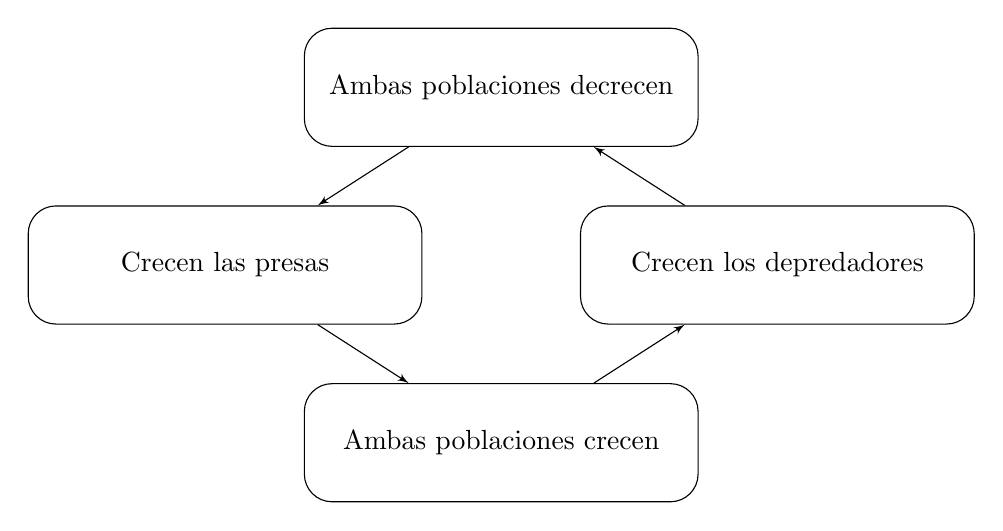
\begin{tikzpicture}[>=latex' ]
        \tikzset{block/.style={draw,
                shape=rectangle,
                align=center,
                rounded corners=1em,
                minimum width=5cm,
                minimum height=1.5cm
            },
        }
        \node [block] (decrecen)
            {Ambas poblaciones decrecen};
        \node [block, below =3cm of decrecen] (crecen)
            {Ambas poblaciones crecen};
        \node [block, below left =1.5cm and =3cm of decrecen] (crecen_p)
            {Crecen las presas};
        \node [block, below right =1.5cm and =-3cm of decrecen] (crecen_d)
            {Crecen los depredadores};
%% paths
\path[draw,->] 
    (decrecen) edge (crecen_p)
    (crecen) edge (crecen_d)
    (crecen_p) edge (crecen)
    (crecen_d) edge (decrecen)
;
\end{tikzpicture}
\end{center}

Podemos ver en este diagrama que aparentemente no hay equilibro entre ambas poblaciones, por el contrario, parece que podrían caer en un ciclo.

\section{Diagrama de fase}

El diagrama de fase es una herramienta que nos permite entender la relación entre las poblaciones. Vamos a aproximar las tasas de crecimiento de ambas poblaciones utilizando el algoritmo de Runge Kutta de 4to orden (RK4), utilizando distintos puntos iniciales (generados al azar utilizando la distribución uniforme) para observar las tendencias en la relación. A su vez, vamos a mostrar en conjunto los vectores que indican la dirección:

\begin{figure}[H]
    \centering
    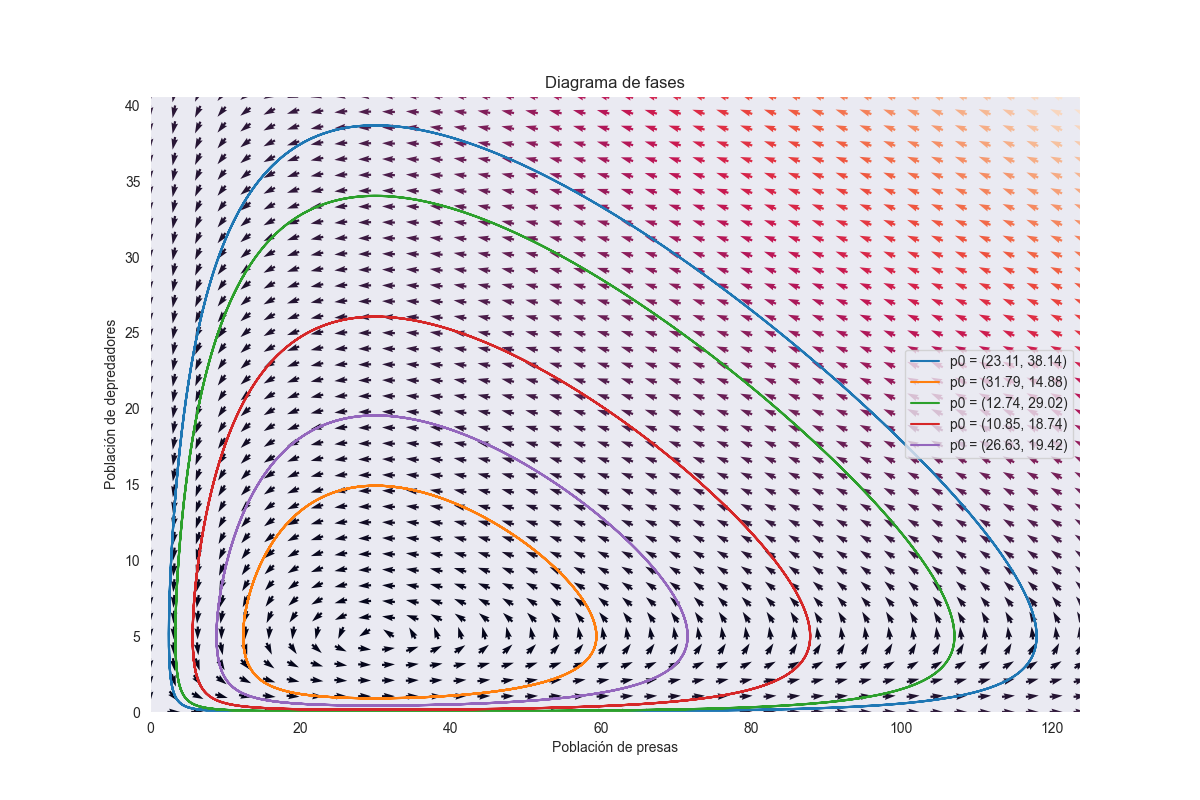
\includegraphics[width=12cm,keepaspectratio]{./diagramas/fases.png}
    \caption{Diagrama de Fase}\label{fig:fase}
\end{figure}

Podemos observar en el grafico \ref{fig:fase} que todos siguen la dirección marcada por el campo de vectores y que en ninguno de los casos las poblaciones se estabilizan, por el contrario, siguen un ciclo.


\section{Evolución a través del tiempo}

Buscamos una solución aproximada (nuevamente usando RK4) utilizando un punto inicial $(40, 9)$ y valores de $t$ en $(0, 200)$. El grafico resultante es:

\begin{figure}[H]
    \centering
    \includegraphics[width=10cm,keepaspectratio]{./diagramas/evolucion.png}
    \caption{Evolución}\label{fig:time}
\end{figure}

Podemos observar en la figura \ref{fig:time} que el crecimiento de ambas poblaciones se corresponde con el descripto en el diagrama de flujo antes mencionado. Además, el modelo no parece estabilizarse en ningún punto, si no que varía constantemente a través del tiempo.

\section{Análisis de Puntos Críticos}

\subsection{Puntos Críticos}

Comenzamos por buscar los puntos críticos del modelo {\bf Lotka-Volterra}. Los puntos críticos también son llamados puntos de equilibro y se definen como los puntos tales que $\dot x = 0$ para una ODE $\dot x = f(x)$. En este caso buscamos puntos tales que $\dot C = 0$ y $\dot Z = 0$. Recordemos que estos no significa que las poblaciones sean nulas, si no que las derivadas son nulas, lo cuál quiere decir que no crecen ni decrecen.

Comenzamos buscando los puntos para $\dot C$, es decir, puntos tales que:

\[ \dot{C} = \alpha C - \beta C Z = 0 \Rightarrow \alpha C = \beta C Z \]

Vemos que hay dos casos para los que esta condición se cumple: $C = 0$ (pues $C$ se encuentra multiplicando ambos términos) y $Z = {\alpha \over \beta}$ (pues reducimos a $\alpha C = \alpha C$).

Por otro lado, consideramos $\dot Z$:

\[ \dot{Z} = - \delta Z + \gamma C Z = 0 \Rightarrow  \delta Z = \gamma C Z \]

Los casos para los que esta condición se cumple son: $Z = 0$ (pues $Z$ se encuentra multiplicando ambos términos) y $C = {\delta \over \gamma}$ (pues reducimos a $\delta Z = \delta Z$).

\pagebreak
Ahora, utilizando estos casos antes mencionados, vemos que los siguientes puntos logran un equilibro conjunto:

\[ (C, Z) = (0, 0) \qquad (C, Z) = ({\alpha \over \beta}, {\delta \over \gamma}) \]

Es fácil ver que $ (C, Z) = (0, {\delta \over \gamma})$ y $ (C, Z) = ({\alpha \over \beta}, 0) $ no son puntos de equilibro.

\subsection{Análisis}

Ahora vamos a linealizar el modelo alrededor de estos puntos, clasificar cada uno y buscar los autovectores. Para lograr esto, deberemos evaluar la matriz jacobina del modelo en los puntos obtenidos $(0, 0)$ y $(30, 5)$. La matriz jacobina del modelo es:

\begin{equation*}
J(C, Z) = 
\begin{pmatrix}
\alpha - \beta Z & - \beta C \\
\delta Z & \delta x - \gamma
\end{pmatrix}
\end{equation*}

Ahora evaluamos esta matriz en los puntos de equilibrio y calculamos los autovalores ({\it eigenvalues}):

\begin{equation*}
J(0, 0) = 
\begin{pmatrix}
0.1 & 0 \\
0 & -0.3
\end{pmatrix}
, \,
\lambda_1 = 0.1
, \,
\lambda_2 = -0.3
\end{equation*}

\begin{equation*}
J(30, 5) = 
\begin{pmatrix}
0 & -0.6 \\
0.05 & 0
\end{pmatrix}
, \,
\lambda_1 = i\sqrt{0.03}
, \,
\lambda_2 = -i\sqrt{0.03}
\end{equation*}

Dados estos autovalores, utilizamos el siguiente criterio para clasificarlos:

\begin{itemize}
    \item{{\bf Estable o Atractor}: cuando los autovalores de la matriz jacobina son reales del mismo signo o complejos cuya parte real es igual}
    \item{{\bf Inestable o Repulsor}: cuando los autovalores de la matriz jacobina son reales de distinto signo}
    \item{{\bf Centro}: cuando los autovalores de la matriz jacobina son imaginarios puros}
\end{itemize}

Vemos que para los puntos de equilibrio que encontramos, ninguno de los dos es un punto estable. Para $(0, 0)$, al tener autovalores reales de distinto signo, podemos concluir que es un punto inestable y esto implica que sólo podemos estabilizarnos en este punto si comenzamos con estos valores iniciales. Por otro lado para el punto $(30, 5)$ obtenemos imaginarios puros, lo cual significa que este es un punto de {\bf centro}, por lo que no podemos concluir nada sobre su estabilidad. Aún así, al observar el diagrama de fases de la figura \ref{fig:fase}, vemos que para los distintos puntos iniciales con los que probamos, la relación se encontraba centrada en el punto $(30, 5)$.

\section{Conclusión}

Realizamos un diagrama de fase para comprender la relación entre ambas poblaciones utilizando distintos puntos iniciales, el cual parecía no tener grandes variaciones y presentaba un comportamiento cíclico. Al realizar un análisis del comportamiento del modelo a través del tiempo, nuevamente vimos que los tamaños de las poblaciones parecía fluctuar continuamente y no estabilizarse. Por último, linealizamos el modelo para analizar los puntos de equilibrio y encontramos que efectivamente, el modelo no tiene puntos estables, por lo que sin importar el punto inicial, siempre va a presentar un comportamiento cíclico..

\end{document}
